\documentclass{csc2059practical}

\setpracticalnumber{3}
\setpracticaltitle{Pointers, Dynamic Arrays, and Manual Memory Management}
\setpracticalsubtitle{Understanding and controlling memory behaviour in C++}
\setpracticalauthor{Dr Giuseppe Trombino, Queen's University Belfast, School of EEECS}
\setpracticaldate{}

\begin{document}

\maketitle
\tableofcontents
\clearpage

\begin{learningoutcomes}
By the end of this practical, you should be able to:
\begin{itemize}
  \item explain the relationship between variables, references, pointers, and memory addresses;
  \item identify unsafe pointer behaviour and explain why it occurs;
  \item use pointers as function parameters to modify caller-owned data;
  \item traverse arrays using indexing and pointer arithmetic;
  \item allocate, resize, and deallocate dynamic arrays safely;
  \item implement concatenation and insertion operations on dynamic arrays;
  \item organise reusable functionality into header and implementation files.
\end{itemize}
\end{learningoutcomes}

\begin{workflowreminder}
This practical follows a simple but important pattern:

\begin{center}
  
\VerticalWorkflowSeven
      {Predict}
      {Observe}
      {Understand}
      {Test}
      {Implement}
      {Refine}
      {Reuse}

\end{center}

Do not treat failing tests as bad news. In this practical, the tests are there to guide your implementation. A failing test is information.
\end{workflowreminder}

\frontsection{Introduction}

In this practical, you will explore how pointers behave through a series of small demonstrations before applying these ideas to dynamic array operations.

The first part of the practical asks you to read short programs, predict what they will do, and then run them. This is deliberate. Before you start manipulating memory directly, you need to be comfortable interpreting what pointers, addresses, and dereferenced values actually mean.

After that, you will use the public tests to guide your implementation of several dynamic array operations. These operations are deliberately low-level: you will allocate memory manually, copy values, update pointers, and release memory when it is no longer needed.

The techniques developed here underpin many of the data structures studied later in CSC2059, including array-backed lists, stacks, queues, and vectors. The aim is to move from \textbf{understanding memory behaviour} to \textbf{controlling memory behaviour}, and then to packaging that behaviour into reusable code.

\begin{infobox}
\textbf{Estimated time:} approximately two hours, including reading, testing and reflection.

Some students will complete the core tasks more quickly, while others will need more time with the pointer and memory-management details. That is normal. Work steadily, run the tests often, and avoid making large untested changes.
\end{infobox}

\frontsection{Before You Begin}

Before starting this practical, complete the Practical 3 self-assessment quiz on Canvas.

The quiz is not intended to punish you. It is there to check that the basic pointer and memory-management ideas are fresh before you start writing code that manipulates memory directly. You may attempt the quiz multiple times.

\begin{importantnote}
You should complete the Canvas self-assessment before beginning the implementation tasks in this practical.
\end{importantnote}

\frontsection{Getting the Practical Repository}

The repository link for this practical will be provided on Canvas. 

Use the Canvas link to accept the Practical 3 assignment in Classroom50. Follow the clone and GitHub sign-in steps from Practical 2, using your registered account and a suitable work folder (on I: in the laboratory). Replace both quoted placeholders below with your actual repository URL and folder name.

\begin{bashcode}
git clone "YOUR_REPOSITORY_URL"
cd "YOUR_REPOSITORY_FOLDER"
code .
\end{bashcode}

\begin{importantnote}
Open the repository root in VS Code. On Windows select the \textbf{CSC2059 Terminal}; on macOS/Linux use the integrated terminal configured in Lab 0. Use the supplied Makefile commands, as in Practical 2.
\end{importantnote}

\begin{commonerror}
If a command such as \texttt{make test-search} fails with a message similar to \texttt{No rule to make target}, check that your terminal is open in the root folder of the repository. This is the folder containing the \texttt{Makefile}.
\end{commonerror}

\frontsection{Repository Tour}

Before editing, look around the repository. Practical 2 kept its header and implementation at the root. This practical groups declarations in \texttt{include/}, implementations in \texttt{src/}, and demonstration programs in \texttt{examples/}. Tests remain in \texttt{tests/}; \texttt{external/} contains the supplied testing library.

\begin{terminal}
external/
    catch.hpp

examples/
    demo01_values_addresses.cpp
    demo02_direct_assignment.cpp
    demo03_indirect_assignment.cpp
    demo04_unsafe_pointers.cpp

include/
    DynamicArrayUtils.h

src/
    DynamicArrayUtils.cpp

tests/
    test_search.cpp
    test_resize.cpp
    test_add.cpp
    test_insert.cpp

Makefile
README.md
\end{terminal}

\begin{infobox}
\textbf{The files you should focus on are:}
\begin{itemize}
  \item \texttt{examples/}: small demonstration programs used in the first part of the practical;
  \item \texttt{include/DynamicArrayUtils.h}: the public function declarations and documentation comments;
  \item \texttt{src/DynamicArrayUtils.cpp}: the file where you will implement the required functions;
  \item \texttt{tests/}: public Catch2 tests that describe the expected behaviour;
  \item \texttt{Makefile}: the build commands used to run demos and tests.
\end{itemize}
\end{infobox}

Most of your implementation work will take place in:

\begin{terminal}
src/DynamicArrayUtils.cpp
\end{terminal}

The function declarations are already provided in:

\begin{terminal}
include/DynamicArrayUtils.h
\end{terminal}

You should read the header file carefully. The comments above each function describe the intended behaviour and will also appear as hints in VS Code.

\frontsection{Build and Test Commands}

Run these commands from the repository root. As in Practical 2, Make builds changed source/header files when needed and puts executables in the ignored \texttt{bin/} folder. On Windows the executable names end in \texttt{.exe}; the Make commands are identical on all three platforms.

\begin{tabularx}{\linewidth}{@{}l X@{}}
\texttt{make} or \texttt{make build} & Build all demos and tests without running them.\\
\texttt{make run} & Build and run all four demonstrations.\\
\texttt{make run-demo01} & Run Demo 01; use \texttt{02}, \texttt{03} or \texttt{04} for the others.\\
\texttt{make test} & Run the core test groups in order; stop at the first failure.\\
\texttt{make test TEST\_MODE=all} & Run all groups for an overview of remaining work.\\
\texttt{make clean} & Remove generated files from \texttt{bin/}; keep your source files.\\
\texttt{make help} & Display the available commands.\\
\end{tabularx}

There are four core test groups: \texttt{test-search}, \texttt{test-resize}, \texttt{test-add} and \texttt{test-insert}. Use a group while implementing its function, then check the others for regressions. For example:
\begin{bashcode}
make test-add
make test-add TEST_MODE=all
\end{bashcode}
The default is \texttt{TEST\_MODE=first}. A setting applies only to the command where you write it. The all mode continues to later test cases and groups after ordinary failures, but still reports failure if any group fails. A compiler error is a build problem; a crash can prevent an executable from completing all its cases. You do not need \texttt{make clean} after ordinary source edits.

\section{Part A - Fundamentals}

\exercise{Pointer Fundamentals}{}

\begin{infobox}
\textbf{Estimated effort:} 15--20 minutes.
\end{infobox}

\begin{learningoutcomes}
In this section, you will:
\begin{itemize}
  \item interpret the relationship between values, variables, addresses, and pointers;
  \item compare direct assignment with indirect assignment through a pointer;
  \item recognise unsafe pointer behaviour before writing larger dynamic-memory code.
\end{itemize}
\end{learningoutcomes}

This exercise is a concept check. You are not expected to implement new functionality here. Instead, read each demonstration program, make a prediction, and then run it.

\subsection{Demo 01: Values and Addresses}

Examine the source code in:

\begin{terminal}
examples/demo01_values_addresses.cpp
\end{terminal}

Before running the program, consider:
\begin{itemize}
  \item What value is stored in \texttt{x}?
  \item What does \texttt{\&x} represent?
  \item Why does every variable have an address?
\end{itemize}

Once you have made your prediction, run:

\begin{bashcode}
make run-demo01
\end{bashcode}

Compare the output with what you expected.

\begin{figure}[htbp]
  \centering
  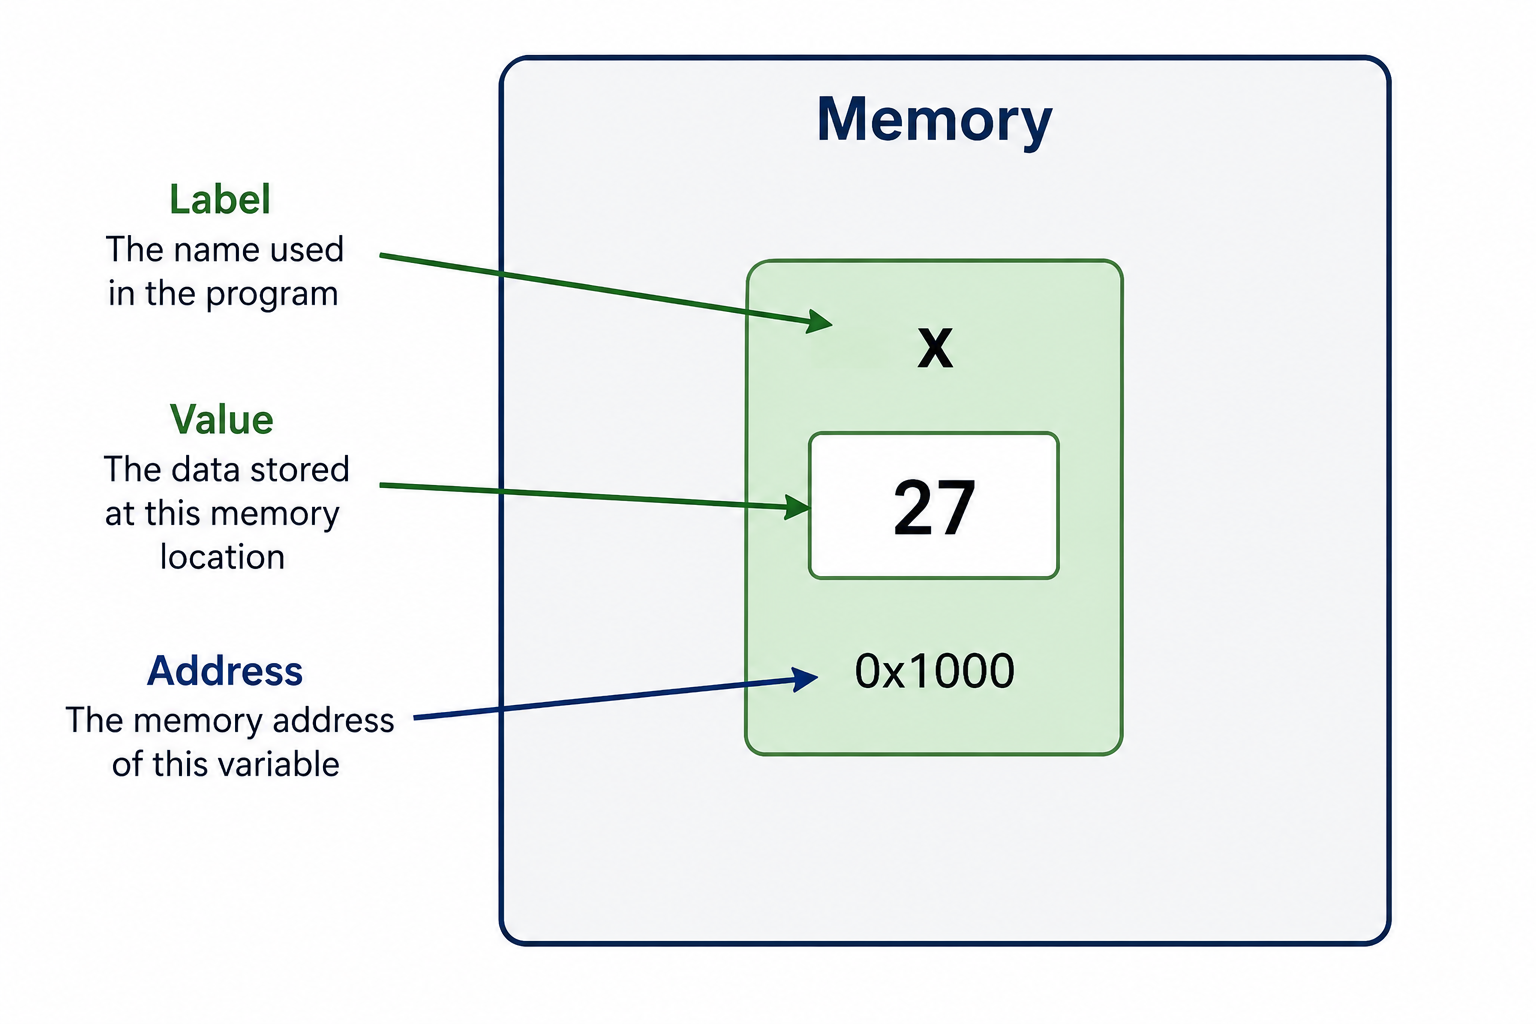
\includegraphics[width=0.7\textwidth]{../../../assets/figures/practical03/var_in_memory.png}
  \caption{Variable in memory}
  \label{fig:VariableInMemory}
\end{figure}

\begin{tipbox}
A useful way to think about this demonstration is that \texttt{x} has two important properties: it stores a value, and it lives somewhere in memory. The expression \texttt{x} gives you the value. The expression \texttt{\&x} gives you the address.
\end{tipbox}

\subsection{Demo 02: Direct Assignment}

Examine the source code in:

\begin{terminal}
examples/demo02_direct_assignment.cpp
\end{terminal}

Before running the program, consider:
\begin{itemize}
  \item What happens when one variable is assigned the value of another?
  \item Does modifying \texttt{y} affect \texttt{x}?
  \item Why does this behaviour make sense?
\end{itemize}

Once you have made your prediction, run:

\begin{bashcode}
make run-demo02
\end{bashcode}

Compare the output with what you expected.


\begin{figure}[htbp]
  \centering
  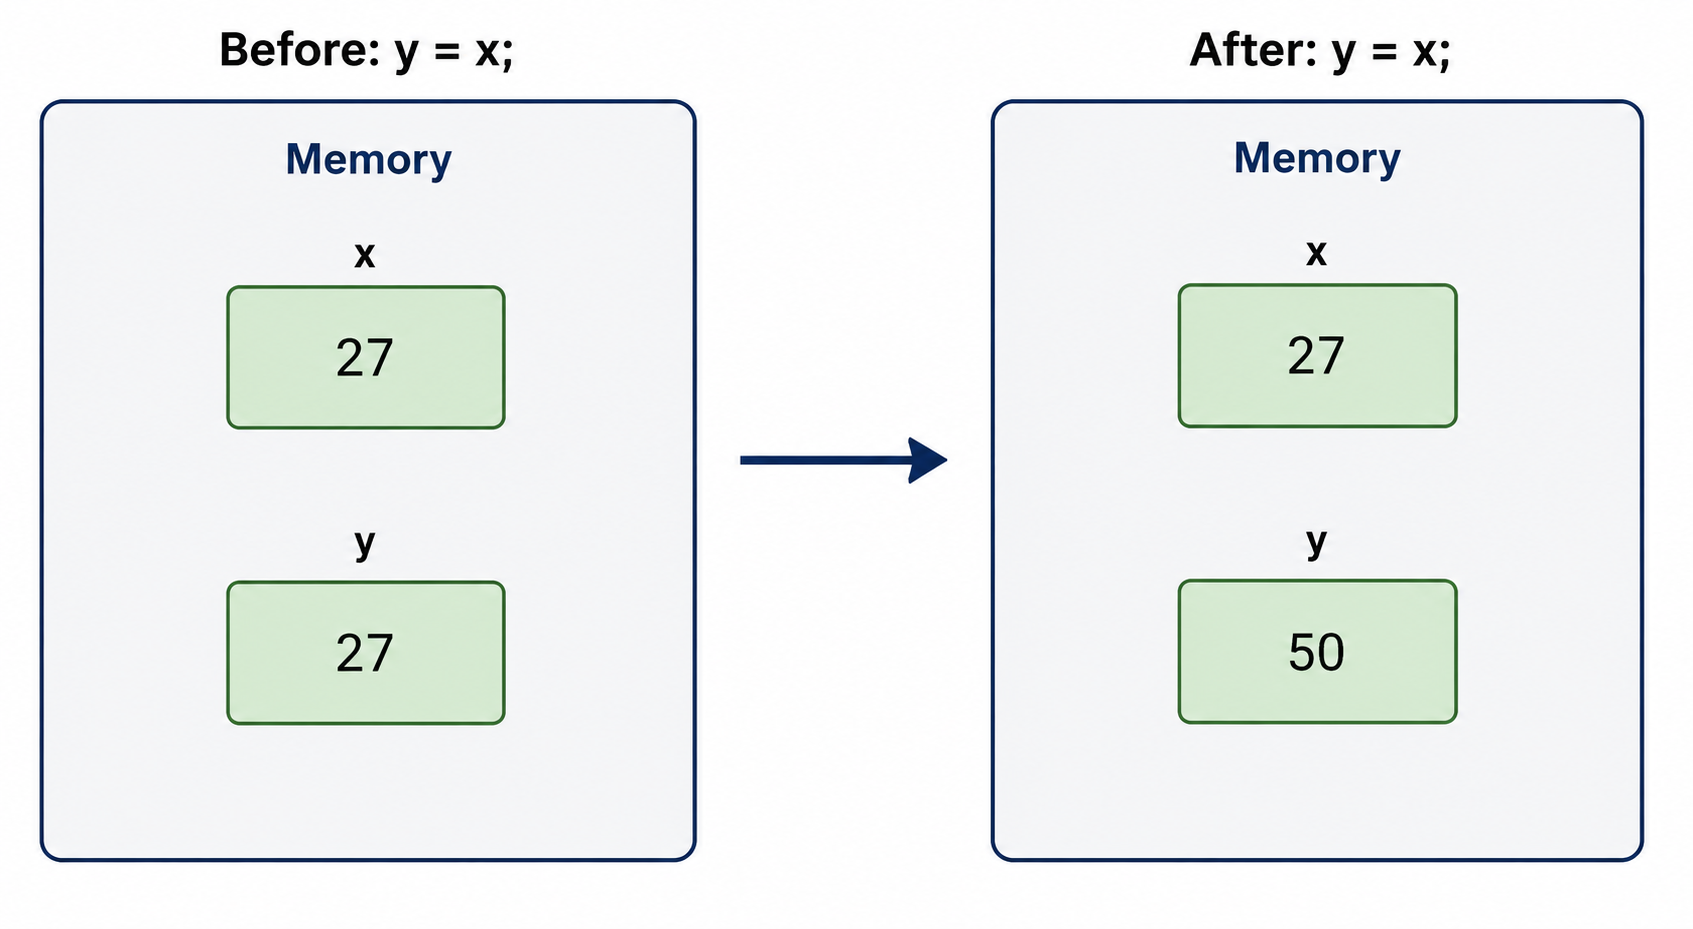
\includegraphics[width=0.9\textwidth]{../../../assets/figures/practical03/direct-assignment.png}
  \caption{Direct Assignment}
  \label{fig:directAssignment}
\end{figure}

\begin{tipbox}
Direct assignment copies a value. After \texttt{int y = x;}, the variables \texttt{x} and \texttt{y} are separate variables. Changing \texttt{y} later does not change \texttt{x}.
\end{tipbox}

\Needspace{70mm}
\subsection{Demo 03: Indirect Assignment}

Examine the source code in:

\begin{terminal}
examples/demo03_indirect_assignment.cpp
\end{terminal}

Before running the program, consider:
\begin{itemize}
  \item What value does the pointer \texttt{p} store?
  \item What does \texttt{*p} represent?
  \item What happens to \texttt{x} when \texttt{*p = 50} is executed?
\end{itemize}

Once you have made your prediction, run:

\begin{bashcode}
  make run-demo03
\end{bashcode}

This is the key idea: a pointer provides another route to an existing object.

\begin{figure}[htbp]
\centering
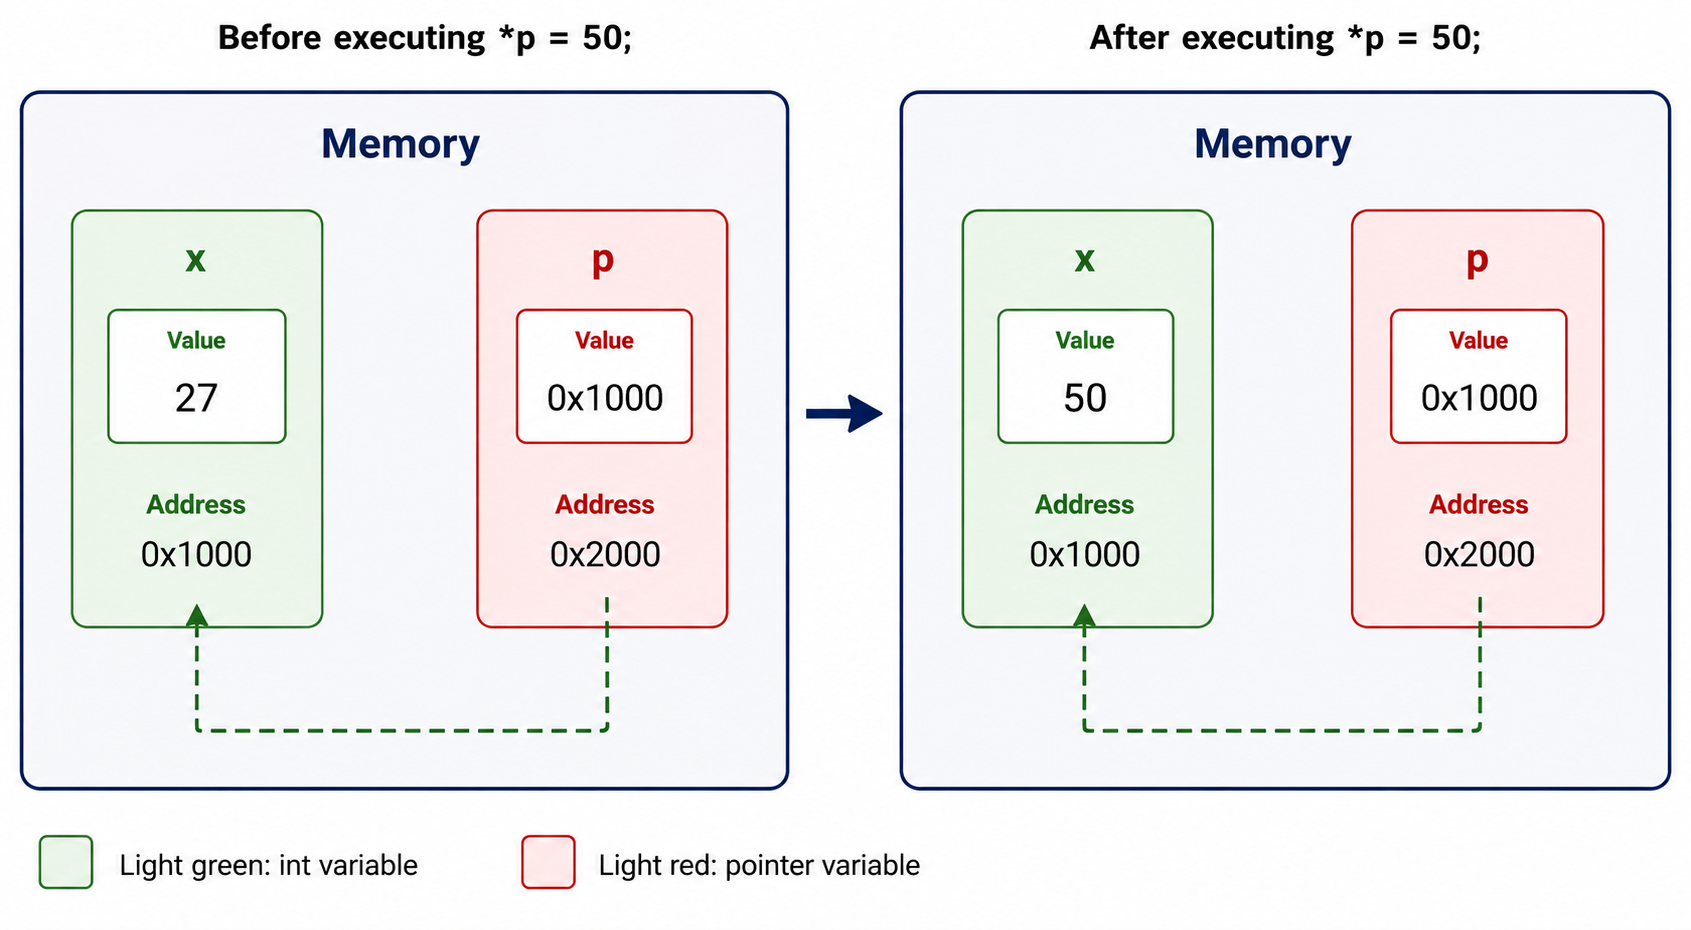
\includegraphics[width=\textwidth]{../../../assets/figures/practical03/indirect_assignment.png}
\caption{Indirect Assignment}
\label{fig:indirectAssignment}
\end{figure}

\begin{tipbox}
The pointer \texttt{p} stores the address of \texttt{x}. The expression \texttt{*p} follows that address and accesses the value stored there. Therefore, assigning to \texttt{*p} changes \texttt{x}.
\end{tipbox}


\Needspace{70mm}
\subsection{Demo 04: Unsafe Pointer Behaviour}

Examine the source code in:

\begin{terminal}
examples/demo04_unsafe_pointers.cpp
\end{terminal}

Before running the program, consider:
\begin{itemize}
  \item Why is dereferencing \texttt{nullptr} unsafe?
  \item What happens to a local variable when a function returns?
  \item Why might a dangling pointer appear to work sometimes, even though the code is still wrong?
\end{itemize}

Once you have made your prediction, run:

\begin{bashcode}
make run-demo04
\end{bashcode}

The file contains two lines of commented-out code. These lines are unsafe on purpose. To see why, uncomment one unsafe line at a time, run \texttt{make run-demo04}, observe what happens, and then comment the line out again before moving on.

\begin{importantnote}
The compiler may warn that \texttt{unsafeCube} returns the address of a local variable. That warning is intentional here. Unsafe pointer behaviour may crash the program, print unexpected output, or appear to work. If the program crashes, that is part of the lesson. Restore the comments before continuing with the rest of the practical.
\end{importantnote}

\begin{commonerror}
Dereferencing a null pointer causes undefined behaviour. Returning the address of a local variable creates a dangling pointer because the local variable ceases to exist when the function exits.
\end{commonerror}
\clearpage
\begin{tipbox}
If a program involving invalid pointer behaviour appears to work once, that does not make it correct. Undefined behaviour is allowed to look correct, crash, print nonsense, or change behaviour between runs.
\end{tipbox}

\section{Part B - Dynamic Arrays}

\exercise{Traversing Dynamic Arrays}{}

\begin{infobox}
\textbf{Estimated effort:} 15--20 minutes.
\end{infobox}

\begin{learningoutcomes}
In this section, you will:
\begin{itemize}
  \item traverse an array using a known size;
  \item count occurrences of a target value;
  \item use public tests to guide a small implementation task.
\end{itemize}
\end{learningoutcomes}

\subsection{From Assertions to Catch2}

Practical 2 used \texttt{assert}, which stops the program at its first failed check. Here, the supplied \texttt{external/catch.hpp} provides \textbf{Catch2 2.13.10}, a test framework that organises checks into named cases and reports failures. It is already in the repository; do not install another copy.

The first case in \texttt{tests/test\_search.cpp} follows this pattern:
\begin{cppcode}
TEST_CASE("search counts one occurrence within the specified size")
{
    char array[] = {'a', 'b', 'c', 'd', 'c'};
    int count = search(array, 4, 'c');
    REQUIRE(count == 1);
}
\end{cppcode}
\texttt{TEST\_CASE} names a behaviour. \texttt{REQUIRE} checks a condition; if it fails, the remainder of that case is skipped. With the default first-failure mode, the run also stops. With \texttt{TEST\_MODE=all}, Catch2 continues to later cases and Make continues to later groups. This does not mean every assertion after a failed \texttt{REQUIRE} will execute.

The supplied test runner provides the test program's \texttt{main}. The Makefile compiles it with your implementation and runs it. For the unfinished \texttt{search}, output will include a failure resembling:
\begin{terminal}
search counts one occurrence within the specified size
REQUIRE( count == 1 )
with expansion:
  0 == 1
\end{terminal}
The case name identifies the behaviour, and \texttt{0 == 1} shows the actual and expected values. Run/read the relevant tests, implement a small change, rerun, and preserve earlier successes. Writing extra tests remains optional.

\subsection{Task 1: Searching in an array}

The first function you will implement is:

\begin{cppcode}
int search(char* array,
           int size,
           char key);
\end{cppcode}

This function returns a \textbf{count}, not an index or a Boolean. It counts how many times \texttt{key} appears in the first \texttt{size} elements of \texttt{array}.

Before writing code, run the tests:

\begin{bashcode}
make test-search
\end{bashcode}

Some tests should fail at this point. That is expected. Read the test names carefully. They describe the behaviour your implementation needs to provide.

Use the tests to guide your implementation in:

\begin{terminal}
src/DynamicArrayUtils.cpp
\end{terminal}

Your implementation should:
\begin{itemize}
  \item count the number of occurrences of \texttt{key};
  \item examine only the first \texttt{size} elements;
  \item return \texttt{0} if \texttt{array} is \texttt{nullptr};
  \item return \texttt{0} if \texttt{size <= 0};
  \item leave the array unchanged.
\end{itemize}

Make one small change, run \texttt{make test-search}, read the result, and repeat until all search tests pass.

\begin{commonerror}
Do not search beyond the first \texttt{size} elements. The array may contain additional values after that point, but this function should ignore them.
\end{commonerror}

\begin{tipbox}
You can access the \texttt{i}-th element using \texttt{array[i]}. You can also use pointer arithmetic with \texttt{*(array + i)}. Both refer to the same element.
\end{tipbox}

\begin{challengebox}
Can you write a second local version of the search algorithm using pointer arithmetic instead of array indexing? Which version do you find easier to read?
\end{challengebox}

\exercise{Managing Dynamic Arrays}{}

\begin{infobox}
\textbf{Estimated effort:} 45--55 minutes.
\end{infobox}

\begin{learningoutcomes}
In this section, you will:
\begin{itemize}
  \item resize dynamically allocated arrays safely;
  \item preserve existing values while moving data into newly allocated memory;
  \item concatenate two dynamic arrays;
  \item insert a value at a specific position in a dynamic array.
\end{itemize}
\end{learningoutcomes}

This exercise is the core of the practical. You will now implement functions that allocate new memory, copy values, update pointers, and release memory that is no longer needed.

\begin{importantnote}
Most dynamic array operations in this practical follow the same pattern:

allocate new memory, copy required values, release old memory, redirect the pointer, and update the size.
\end{importantnote}

\begin{infobox}
\textbf{Why do these parameters contain \texttt{\&}?}

A C++ reference is an alias for an existing variable. An \texttt{int\& size} parameter lets a function update the caller's size variable. An \texttt{int*\& array} parameter is a reference to the caller's pointer: assigning to \texttt{array} replaces that pointer. The \texttt{char*\&} form does the same for a character-array pointer.

This differs from assigning to \texttt{array[i]}, which changes an element. After allocating a replacement array, the function must redirect the caller's pointer to it and update the caller's size. Pass the pointer and size variables directly, for example \texttt{resizeArray(values, size, 5)}; do not add an extra \texttt{\&} at the call.
\end{infobox}

The current array passed to \texttt{resizeArray} or \texttt{insert} must be a valid \texttt{new[]} allocation with its recorded size, or \texttt{nullptr} with size zero. The function takes responsibility for releasing the old allocation when it replaces it; the caller eventually deletes the final array.

\subsection{Task 2: Resizing Arrays}

The next function is:

\begin{cppcode}
bool resizeArray(int*& array,
                 int& size,
                 int newSize);
\end{cppcode}

Start by running the tests:

\begin{bashcode}
make test-resize
\end{bashcode}

Several tests should fail initially. Use those failures as your guide. Read the test names first, then make one small implementation change and run the tests again.

Your implementation should:
\begin{itemize}
  \item return \texttt{false} if \texttt{newSize < 0};
  \item preserve existing values when resizing succeeds;
  \item initialise new elements to \texttt{0} when expanding;
  \item keep only the values that fit when shrinking;
  \item treat \texttt{newSize == 0} as deleting the array;
  \item set \texttt{array} to \texttt{nullptr} and \texttt{size} to \texttt{0} when deleting the array;
  \item leave the original array and size unchanged if resizing fails.
\end{itemize}

Implement the function gradually. Run \texttt{make test-resize} after each meaningful change.

\begin{commonerror}
Do not delete the original array before copying its contents. Once the old memory has been released, the values stored there are no longer yours to use.
\end{commonerror}

\begin{commonerror}
Forgetting to release the old array after a successful resize causes a memory leak. Every successful \texttt{new[]} should eventually be paired with \texttt{delete[]}.
\end{commonerror}

\begin{tipbox}
A good order is usually: validate inputs, handle the zero-size case, allocate the new array, copy the values that should survive, initialise any new elements, delete the old array, then update the pointer and size.
\end{tipbox}

\subsection{Task 3: Concatenating Arrays}

The next function is:

\begin{cppcode}
bool addArrays(char*& array,
               int& size,
               char* other,
               int otherSize);
\end{cppcode}

Start by running the tests:

\begin{bashcode}
make test-add
\end{bashcode}

The two input ranges must be separate: do not pass the same array, or a pointer into the first array, as \texttt{other}. A nonempty first array must have been allocated with \texttt{new[]}. The function owns neither the second array nor its storage; it copies its values and must not delete it.

Your implementation should:
\begin{itemize}
  \item append the contents of \texttt{other} to the end of \texttt{array};
  \item update \texttt{size} to the combined size;
  \item leave \texttt{other} unchanged;
  \item after validating the inputs, treat \texttt{otherSize == 0} as a valid no-op which keeps the first pointer unchanged;
  \item handle an empty first array;
  \item return \texttt{false} if either size is negative, or if a pointer is \texttt{nullptr} while its corresponding size is greater than zero. A \texttt{nullptr} with size zero is treated as a valid empty array;
  \item leave the original array and size unchanged if the operation fails.
\end{itemize}

Run \texttt{make test-add} frequently as you work.

\begin{commonerror}
The second array should not be modified. This function appends a copy of its values onto the first array.
\end{commonerror}

\begin{tipbox}
This function is a close cousin of \texttt{resizeArray}. You still need to allocate a new array, copy values into it, delete the old first array, and update the pointer.
\end{tipbox}

\subsection{Task 4: Inserting Values}

The final core function is:

\begin{cppcode}
bool insert(int*& array,
            int& size,
            int position,
            int value);
\end{cppcode}

Start by running the tests:

\begin{bashcode}
make test-insert
\end{bashcode}

The valid insertion range is:

\begin{terminal}
0 <= position <= size
\end{terminal}

This means that inserting at position \texttt{0} places the new value at the beginning, while inserting at position \texttt{size} appends the value to the end.

Your implementation should:
\begin{itemize}
  \item reject invalid positions;
  \item allocate a new array with one extra element;
  \item copy all values before the insertion position;
  \item place the new value at the insertion position;
  \item shift the remaining values one place to the right;
  \item update \texttt{size};
  \item leave the original array and size unchanged if insertion fails.
\end{itemize}

Run \texttt{make test-insert} frequently as you work.

\begin{commonerror}
Insertion positions range from \texttt{0} to \texttt{size} inclusive. A position greater than \texttt{size} is invalid.
\end{commonerror}

\begin{commonerror}
Be careful when copying elements after the insertion position. The destination index is one place ahead of the source index.
\end{commonerror}

\begin{tipbox}
Think of insertion as copying the old array in two pieces: everything before the insertion point, then everything from the insertion point onwards shifted one position to the right.
\end{tipbox}

\begin{challengebox}
If you finish the core tasks early, try designing and implementing a complementary function:

\begin{cppcode}
bool remove(int*& array,
            int& size,
            int position);
\end{cppcode}

The function should remove the value at the specified position, shrink the array by one, and preserve the remaining values.
\end{challengebox}

\Needspace{90mm}
\section{Part C - Reflections}

\exercise{Understanding the Utility Library}{}

\begin{infobox}
\textbf{Estimated effort:} 5--10 minutes.
\end{infobox}

\begin{learningoutcomes}
In this section, you will:
\begin{itemize}
  \item recognise the role of header and implementation files;
  \item understand how related functions can be grouped into a reusable component;
  \item connect this practical with the modular structure introduced in earlier work.
\end{itemize}
\end{learningoutcomes}

You have been working with a small utility library throughout this practical:

\begin{terminal}
include/DynamicArrayUtils.h
src/DynamicArrayUtils.cpp
\end{terminal}

The header file contains the public interface: the function declarations and comments describing what each function is expected to do.

The source file contains the implementation: the actual code that makes those functions work.

Take a moment to consider:
\begin{itemize}
  \item Why are declarations placed in a header file?
  \item Why are implementations placed in a source file?
  \item How could another program reuse these functions?
  \item What advantages does this separation give us as programs become larger?
\end{itemize}

\begin{reflectionbox}
This practical began with small demonstrations about values, addresses, and pointers. It then moved into dynamic arrays, resizing, concatenation, and insertion.

That progression matters. Before you can build larger data structures, you need to understand how memory is accessed, copied, resized, and released.
\end{reflectionbox}

\section{Part D - Challenges}

\frontsection{Fast Finisher Challenges}

If you complete the core practical early, you can try one or more of the following optional challenges.

\begin{challengebox}
\textbf{Pointer arithmetic search.} Implement a second local version of \texttt{search()} using pointer arithmetic rather than array indexing. Compare the two versions for readability.
\end{challengebox}

\begin{challengebox}
\textbf{Memory leak investigation.} Temporarily comment out one \texttt{delete[]} statement in your implementation and think through what memory is no longer being released. Restore the correct code afterwards.
\end{challengebox}

\begin{challengebox}
\textbf{Remove operation.} Design a \texttt{remove()} function for dynamic arrays. What should happen if removing the last element reduces the size to zero?
\end{challengebox}

\begin{challengebox}
\textbf{Test design.} Add one extra local Catch2 test for each implemented function. Try to choose a boundary case not already covered by the public tests.
\end{challengebox}

\section{Submission Checklist and Wrap up}

Before finishing the practical, make sure that:

\begin{itemize}
  \item all four demonstrations run with Demo 04's unsafe lines restored to comments;
  \item \texttt{make test-search} passes;
  \item \texttt{make test-resize} passes;
  \item \texttt{make test-add} passes;
  \item \texttt{make test-insert} passes;
  \item \texttt{make test TEST\_MODE=all} confirms that all four core groups pass;
  \item your implementations compile without avoidable warnings (Demo 04 has an intentional warning);
  \item dynamically allocated memory is released appropriately;
  \item your changes have been committed and pushed.
\end{itemize}

Save your files and inspect the changed filenames. The supplied \texttt{.gitignore} excludes \texttt{bin/}; stage only intended source changes and inspect the staged diff. Check your latest commit and author on GitHub after pushing, as in Practical 2.

\begin{bashcode}
git status
git add .
git diff --staged
git commit -m "Complete Practical 3 dynamic array functions"
git push
\end{bashcode}

\begin{wrapupbox}
You have now moved from observing pointer behaviour to implementing dynamic memory operations yourself. This is the groundwork for understanding how many array-backed data structures operate internally. Later in the module, higher-level containers will make some of this work easier, but the ideas you practised here are the machinery underneath.
\end{wrapupbox}

\end{document}
